\documentclass[12pt]{article}
\usepackage[utf8]{inputenc}
\usepackage[margin=1in]{geometry}
\usepackage{amsmath}
\usepackage{graphicx}
\usepackage{enumerate}
\graphicspath{ {./images/} }

\author{Neelu Saraswatibhatla (srns2)}
\title{Operating Systems Supervision 1}
\date{\vspace{-5ex}}

\begin{document}

\maketitle

\section{Example Sheet 1}
\begin{enumerate}
      \item \begin{enumerate}
                  \item \begin{enumerate}
                              \item Cache memory is a small amount of high-performance storage that is faster for the processor to access than main memory. The computer uses it to temporarily store data that the processor can retrieve easily.
                              \item Main memory is the main RAM in a computer and it is where files that are currently in use by processes are stored.
                              \item Registers are very fast pieces of memory located on the chip itself. Data is loaded from main memory (or cache memory) onto registers to be operated upon, and then loaded back onto main or cache memory.
                        \end{enumerate}
                  \item If the size of the data being used by processes in progress exceeds the size of main memory, then some of that data is offloaded into disk storage temporarily.
            \end{enumerate}
      \item \begin{enumerate}
                  \item \begin{enumerate}
                              \item An unsigned integer is simply stored as a binary number directly corresponding to the decimal representation of the unsigned integer.
                              \item A signed integer is generally stored as a twos-complement integer. The most significant bit represents the sign (0 is positive, 1 is negative) and the remaining bits represent the value (but not directly). To convert from $x$ to $-x$, invert every bit (including the MSB, turning the integer from positive to negative) and add 1.
                              \item Memory can only store binary strings so a text string has to be converted into binary. The two main standards for this are ASCII and Unicode. ASCII is a 7-bit code that holds American letters, numbers, punctuation, and some other characters. Unicode is an 8-, 12-, or 32-bit code that aims to support all characters and symbols in every language and used by anyone.
                              \item An instruction comprises of an opcode (specifies what operation to perform), zero or more operands (registers where values used in the operations the stored), and the register into which to put the result.
                        \end{enumerate}
                  \item If it wants to interpret the contents of the register and convert them into a human-readable decimal number, for example, then it would need to know whether or not the integer is unsigned. However if it is simply adding or subtracting two integers then it does not need to know this information as adding or subtracting integers is done using the same method for both signed and unsigned integers, adding or subtracting 1.
                  \item During a context switch, the operating system saves the state of a thread, restores the state of another thread, and also switches process state if the two threads were in different processes. Then when context switching back into this first thread, the state ('context') of the thread is restored.
            \end{enumerate}
      \item \(\)\\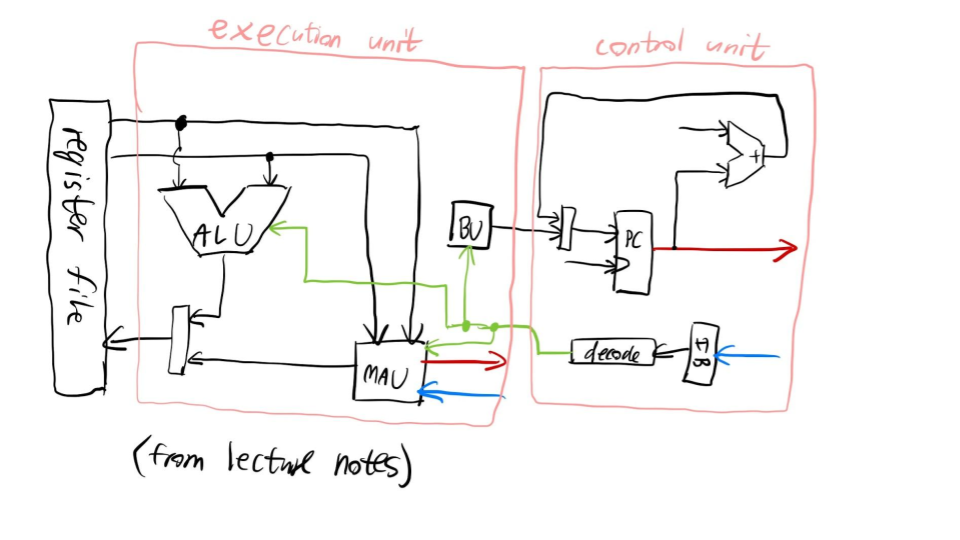
\includegraphics[scale=0.5]{1-q3.png} In each iteration of a fetch-execute cycle, first the CPU fetches and decodes the next instruction, and it then executes it. In the execution unit, control signals select the functional unit required and the operation. There are several functional units, such as: \begin{itemize}
            \item the \textbf{arithmetic logic unit (ALU)}, which reads one or two registers, performs the arithmetic operation, and writes the result into a register.
            \item the \textbf{branch unit (BU)}, which reads one or two registers, tests a condition, and adds a value to the program counter (PC).
            \item the \textbf{memory access unit (MAU)}, which generates an address and uses a bus to read/write a value.
      \end{itemize}
      This is then repeated
      \item With non-preemptive process scheduling, a scheduling decision is only taken when a running processes blocks or terminates, while with preemptive process scheduling, a scheduling decision can be taken when a timer expires or a waiting process unblocks in addition to these.

            Non-preemptive scheduling is simpler to implement that preemptive as the OS only needs to make a decision when a process blocks or terminates so does not need to be constantly doing anything, while preemptive is more complex as the OS needs to be watching for waiting processes unblocking and needs to have a timer.

            Non-preemptive is less fair than preemptive as a longer running process could stop a lot of other shorter process from running, while preemptive allows more processes to be given running time by temporarily stopping a longer process. For the same reason, preemptive offers better performance than non-preemptive.

            Non-preemptive is open to denial-of-service, so a process could just refuse to block or terminate, stopping the computer from doing anything else entirely. Preemptive has a timer so the OS can watch for this.

            By virtue of non-preemptive being simpler, it has fewer hardware requirements, while preemptive has more hardware requirements for things such as the timer.
      \item \begin{enumerate}
                  \item Each job is given a priority (multiple jobs can have the same priority), which is an integer, and the smaller the integer the higher the priority. Every time the CPU makes a scheduling decision (on process blocking/termination in non-preemptive scheduling, or one of these two or timer expiry/waiting process unblocking in preemptive scheduling), it selects the job with the highest priority to run. If multiple jobs have the same priority, then ties can be broken using a round robin with time-slicing, allocating quanta to each process with the same highest priority.
                  \item \begin{itemize}
                              \item FCFS is a priority scheduling algorithm with jobs that arrived first having higher priority (e.g. priority = time of arrival). This is a static priority scheduling algorithm as the time a job arrived never changes.
                              \item Shortest job first is a priority scheduling algorithm with jobs of shortest time required having highest priority (e.g. priority = time required). This is a static priority scheduling algorithm as the total time a job requires never changes.
                              \item Shortest time remaining is a priority scheduling algorithm with jobs of shortest remaining time required having highest priority (e.g. priority = remaining time required). This is a dynamic priority scheduling algorithm as the time remaining of a job can change, e.g. when the process blocks and then unblocks or when a new job that requires shorter time is created.
                              \item Round robin is a dynamic priority scheduling algorithm, with the job currently running having highest priority, and then as soon as its quantum expires, giving it lowest priority and increasing every other job's priority evenly.
                        \end{itemize}
                  \item The biggest problem with static priority scheduling is starvation, as a low priority process is not guaranteed to ever run. A solution is to use a dynamic priority scheduling algorithm, where the priority of a process increases after it has starved for a given amount of time.
                  \item Many CPU scheduling algorithms try to favour IO intensive jobs as they block more often waiting for IO, which allows more jobs to run.
            \end{enumerate}
      \item \begin{enumerate}
                  \item It is being used on a time-sharing system, with many jobs needing to be done.
                  \item Since the algorithm gives each job a certain amount of time on a rotating basis, all jobs are equally prioritised (based on priorities) rather than longer ones stopping other ones from being done, so one user running a long process won't stop the other users from getting anything done.
                  \item \begin{itemize}
                              \item $P_1: 15 - 0 = 15$
                              \item $P_2: 10 - 1 = 9$
                              \item $P_3: 12 - 7 = 5$
                        \end{itemize}
                        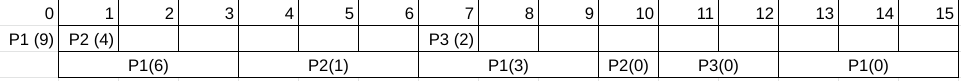
\includegraphics[scale=0.4]{1-roundrobin.png}
                  \item An advantage of using a small quantum is that it is more fair, giving more jobs the chance to run and allowing newer jobs to start running sooner. A disadvantage, however, is that context switching is not instant, so every time the current process is changed to a different one (and therefore context switching occurs), the CPU wastes time not doing any useful work.
            \end{enumerate}
      \item \begin{enumerate}
                  \item \(\)\\ 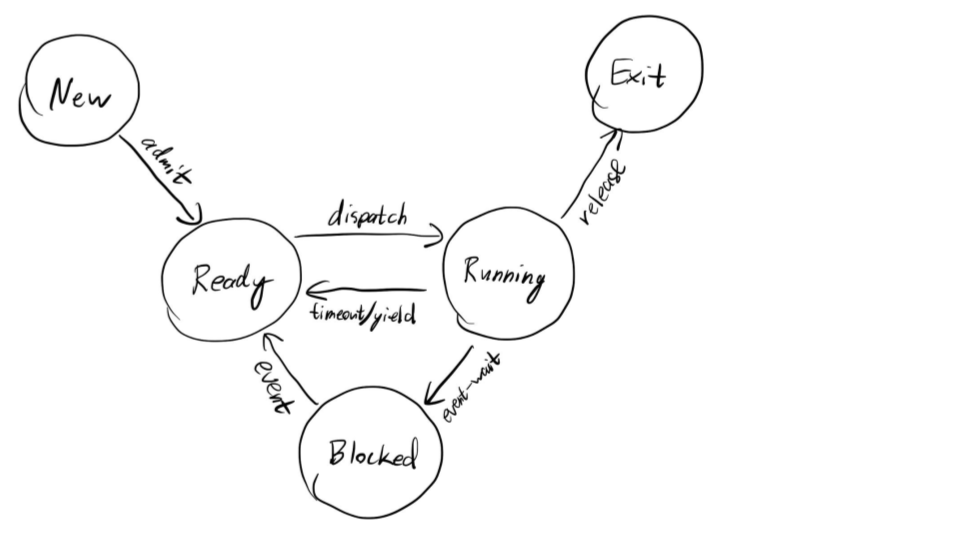
\includegraphics[scale=0.5]{1-q7a} When a process is created, it starts in the New state. It then goes to the Ready state (the admit transition) when it is ready to be run by the CPU. It then goes from Ready to Running (the dispatch transition) when it is allocated run time on the CPU and is being run. It then has multiple possible transitions:
                        \begin{itemize}
                              \item It can go to Blocked (the event-wait transition) while it is waiting for an event, such as I/O.
                              \item It can go back to the Ready state (the timeout/yield transition) when it yields or its time slice expires.
                              \item It can go to the Exit state (the release transition) when it has finished executing.
                        \end{itemize}
                        In the Blocked state, the program waits for an event. Once that event occurs, it can enter the Running state (event transition) upon OS approval.

                        Once a program has gone into the Exit state, it terminates.
                  \item In the process control block, the OS keeps information about the process such as: \begin{itemize}
                              \item \textbf{Process ID}
                              \item \textbf{Process State}
                              \item \textbf{CPU Shceduling information}
                              \item \textbf{References to previous and next process control blocks}
                              \item \textbf{Other information such as CPU time used so far, identity of owner, list of open files, etc.}
                              \item the \textbf{program counter}, which keeps track of which instruction is being run
                              \item \textbf{general purpose registers} which is where the process puts data it is working on
                              \item \textbf{process status register}
                        \end{itemize}
                  \item It needs to know how long each process requires (in total for SJF, remaining for SRTF). We can estimate this using the amount of time each previous burst took. We can use the formula $\tau_{n+1} = \alpha t_n + \cdots + (1 - \alpha)^j t_{n-j} + (1-\alpha)^{n+1} \tau_0$, where $tau_{n+1}$ is the estimate for the amount of time the next CPU burst ($n+1$) will take, $t_i$ is the amount of time the $i^\text{th}$ burst took, and $\alpha$ is a constant between 0 and 1. We can shorten this and only take terms up to a certain $n - j$ depending on how far back we think provides useful information for future bursts.
                  \item An advantage of non-preemptive scheduling is that it is simpler to implement than preemptive scheduling as we don't need to implement a timer, but a disadvantage is that it is open to denial-of-service by a process that doesn't ever block or terminate, as the OS doesn't step in.
                  \item When an interrupt occurs, in the case of I/O the CPU scheduler decides whether to keep running the current process, or to switch to the process the I/O is intended for. In the case of DMA, the associated data from memory is passed to the process if it has rights to it.
                  \item With too many interrupts, the CPU would be wasting too much time handling them and making decisions about them and spends less time doing useful work. 
            \end{enumerate}
\end{enumerate}

\section{Tripos Question 2012/II/3}
\begin{enumerate}[(a)]
      \item \begin{enumerate}[(i)]
                  \item This mechanism is called context switching, and it involves storing the state of a thread and restoring the state of a different thread (and also process state if the threads are of different processes).
                  \item One method is to save all of the current memory space elsewhere, and then load all of this back when restoring. This is absolute addressing and does not require virtual addressing, however it takes more time and may not be necessary for processes without high memory requirements. Another method is by using virtual addressing, translating any memory address requested by the process into the actual place in memory it is stored, allowing multiple processes to store data in memory at the same time, and only moving this off memory if the memory gets full.
                  \item Two other elements of the process context are the program counter and page tables.
            \end{enumerate}
      \item \begin{enumerate}
                  \item It gets interrupted (i), then goes straight to ready (g) as it isn't waiting for anything, and the the routine then decides its time slice hasn't expired, so it goes back to running (h). The process scheduler does not need to be run.
                  \item It gets interrupted (i), then once goes straight to ready (g) as it isn't waiting for anything. This time, it stays in the ready state as its time slice has expired so a different process runs instead, and it waits in the ready state until it gets a new time slice. The process scheduler needs to run to determine which process to schedule next.
                  \item It goes from running to kernel (b), and is serviced immediately, going straight back to running (a). The process scheduler does not need to be run.
                  \item It goes from running to kernel (b), to waiting (c) for an I/O operation to be initiated. At this point, the process scheduler needs to be run to determine what to schedule next while this process is waiting for I/O.
            \end{enumerate}
\end{enumerate}

\section{Tripos Question 2010/II/3b}
\begin{enumerate}[(i)]
      \item \(\)\\ 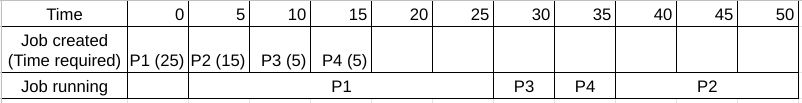
\includegraphics[scale=0.5]{3-sjf.png}\\\\
            $\text{average waiting time} = \dfrac{(25 - 25) + (50 - 20) + (30 - 15) + (35 - 20)}{4} = 15$
      \item \(\)\\ 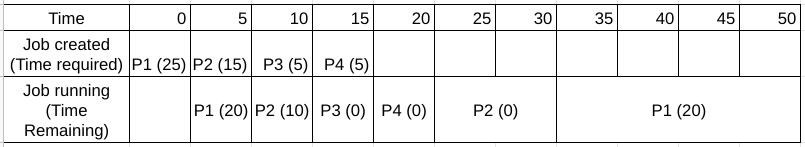
\includegraphics[scale=0.5]{3-srtf.png}\\\\
            $\text{average waiting time} = \dfrac{(50 - 25) + (30 - 20) + (15 - 15) + (20 - 20)}{4} = 8.75$
      \item \(\)\\ 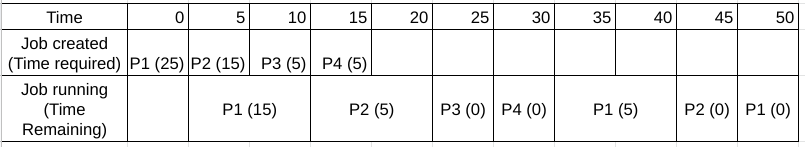
\includegraphics[scale=0.5]{3-rr.png}\\\\
            $\text{average waiting time} = \dfrac{(50 - 25) + (45 - 20) + (25 - 15) + (30 - 20)}{4} = 17.5$
      \item (As above in Example Sheet 1 question 6d) An advantage of using a small quantum is that it is more fair, giving more jobs the chance to run and allowing newer jobs to start running sooner. A disadvantage, however, is that context switching is not instant, so every time the current process is changed to a different one (and therefore context switching occurs), the CPU wastes time not doing any useful work.
\end{enumerate}

\end{document}
